\documentclass[11pt,]{article}
\usepackage[margin=1in]{geometry}
\newcommand*{\authorfont}{\fontfamily{phv}\selectfont}
\usepackage[]{mathpazo}
\usepackage{abstract}
\renewcommand{\abstractname}{}    % clear the title
\renewcommand{\absnamepos}{empty} % originally center
\newcommand{\blankline}{\quad\pagebreak[2]}

\providecommand{\tightlist}{%
  \setlength{\itemsep}{0pt}\setlength{\parskip}{0pt}} 
\usepackage{longtable,booktabs}

\usepackage{parskip}
\usepackage{titlesec}
\titlespacing\section{0pt}{12pt plus 4pt minus 2pt}{6pt plus 2pt minus 2pt}
\titlespacing\subsection{0pt}{12pt plus 4pt minus 2pt}{6pt plus 2pt minus 2pt}

\titleformat*{\subsubsection}{\normalsize\itshape}

\usepackage{titling}
\setlength{\droptitle}{-.25cm}

%\setlength{\parindent}{0pt}
%\setlength{\parskip}{6pt plus 2pt minus 1pt}
%\setlength{\emergencystretch}{3em}  % prevent overfull lines 

\usepackage[T1]{fontenc}
\usepackage[utf8]{inputenc}

\usepackage{fancyhdr}
\pagestyle{fancy}
\usepackage{lastpage}
\renewcommand{\headrulewidth}{0.3pt}
\renewcommand{\footrulewidth}{0.0pt} 
\lhead{}
\chead{}
\rhead{\footnotesize Biology 3103 : Ecology Laboratory -- Fall 2018}
\lfoot{}
\cfoot{\small \thepage/\pageref*{LastPage}}
\rfoot{}

\fancypagestyle{firststyle}
{
\renewcommand{\headrulewidth}{0pt}%
   \fancyhf{}
   \fancyfoot[C]{\small \thepage/\pageref*{LastPage}}
}

%\def\labelitemi{--}
%\usepackage{enumitem}
%\setitemize[0]{leftmargin=25pt}
%\setenumerate[0]{leftmargin=25pt}




\makeatletter
\@ifpackageloaded{hyperref}{}{%
\ifxetex
  \usepackage[setpagesize=false, % page size defined by xetex
              unicode=false, % unicode breaks when used with xetex
              xetex]{hyperref}
\else
  \usepackage[unicode=true]{hyperref}
\fi
}
\@ifpackageloaded{color}{
    \PassOptionsToPackage{usenames,dvipsnames}{color}
}{%
    \usepackage[usenames,dvipsnames]{color}
}
\makeatother
\hypersetup{breaklinks=true,
            bookmarks=true,
            pdfauthor={ ()},
             pdfkeywords = {},  
            pdftitle={Biology 3103 : Ecology Laboratory},
            colorlinks=true,
            citecolor=blue,
            urlcolor=blue,
            linkcolor=magenta,
            pdfborder={0 0 0}}
\urlstyle{same}  % don't use monospace font for urls


\setcounter{secnumdepth}{0}

\usepackage{longtable}

\usepackage{graphicx}
% We will generate all images so they have a width \maxwidth. This means
% that they will get their normal width if they fit onto the page, but
% are scaled down if they would overflow the margins.
\makeatletter
\def\maxwidth{\ifdim\Gin@nat@width>\linewidth\linewidth
\else\Gin@nat@width\fi}
\makeatother
\let\Oldincludegraphics\includegraphics
\renewcommand{\includegraphics}[1]{\Oldincludegraphics[width=\maxwidth]{#1}}



\usepackage{setspace}

\title{Biology 3103 : Ecology Laboratory}
\author{Stephen Cook \& Dr.~Robert Doyle}
\date{Fall 2018}


\begin{document}  

		\maketitle
		
	
		\thispagestyle{firststyle}

%	\thispagestyle{empty}


	\noindent \begin{tabular*}{\textwidth}{ @{\extracolsep{\fill}} lr @{\extracolsep{\fill}}}


E-mail: \texttt{\href{mailto:stephen_cook@baylor.edu}{\nolinkurl{stephen\_cook@baylor.edu}},
\href{mailto:robert_doyle@baylor.edu}{\nolinkurl{robert\_doyle@baylor.edu}}} \\
Office Hours: MTu 9:00-11:00am (Cook), or by appointment  &  Class Hours: 2:00-6:15\\
Office: C453.R (Cook), C419 (Doyle)  & Class Room: A222\\
	&  \\
	\hline
	\end{tabular*}
	
\vspace{2mm}
	


\section{Course Objectives}\label{course-objectives}

The goal of this lab is to develop the student as a scientist by
exposure to basic research methodology in the field of ecology. You will

\begin{enumerate}
\def\labelenumi{\arabic{enumi}.}
\item
  develop understanding of ecology as a scientific discipline, and
\item
  become familiar with some common methods used by ecologists (including
  field, laboratory, and data handling practices).
\end{enumerate}

\section{General information}\label{general-information}

Ecology is synonymous with field research - barring dangerous conditions
(e.g., lightning) we will be outdoors if the planned lab is outdoors.
Rain or shine! Wearing clothes not suited to field conditions will not
be considered a valid excuse to not participate in the lab, so dress
appropriately.

In the lab, university policy is that you must wear closed-toe shoes and
long pants. Pay attention to the weather and dress appropriately for
outdoor conditions! For the wet labs I would wear old jeans or quick-dry
pants/shorts. Shorts could be fine- but we may be wading through
vegetation (scratchy). Old tennis shoes are highly recommended. You will
not be allowed to wade barefoot (i.e., you will not participate in that
lab, and lose participation points). More specific info will be provided
for each outdoor lab.

If you ever have questions or concerns, please do not hesitate to email
either Stephen (preferably) or Dr.~Doyle. We generally respond quickly
to emails, with the exception of the evening before lab reports are due
(Stephen will respond to report questions up untill 5:00pm the day
before the assigment is due). Please take advantage of office hours, and
we are always happy to arrange alternative times to meet if the posted
hours do not work with your schedule.

\subsection{Laboratory/field
activities}\label{laboratoryfield-activities}

It is important that students be aware that participating in laboratory
activities carries the risk, however small, of injury. Should you become
injured during activities in this class, be aware of the following:

\begin{itemize}
\tightlist
\item
  Notify your instructor immediately if you are injured or exposed to a
  chemical. Ask your instructor to provide the chemical safety data
  sheet (SDS) to take with you.
\item
  The Student Health Center can treat minor physical injuries such as
  cuts, burns, etc. The Health Center is open during campus business
  hours. After-hours medical care should be sought at an off-campus
  emergency care facility.
\item
  The Health Center does not provide emergency care for eye injuries or
  chemical exposures. In such cases, treatment should be sought at an
  emergency care center.
\item
  The nearest 24/7 emergency care center is Premier located at 221 N.
  Jack Kultgen Expy (254) 537-9452. Other nearby ERs include BSWMC
  Hillcrest and Express ER.
\item
  Depending on the type/extent of injury, an ambulance may be requested.
\item
  Medical expenses incurred as a result of a laboratory injury,
  including ambulance transport, are the financial responsibility of the
  student.
\end{itemize}

\section{Grading}\label{grading}

\subsection{Point breakdown}\label{point-breakdown}

\begin{itemize}
\item
  \textbf{72 points} - 6 lab reports at 12 points each
\item
  \textbf{18 points} - 6 R scripts at 3 points each
\item
  \textbf{10 points} - 2 field trips at 5 points each
\end{itemize}

\subsection{Grading scale}\label{grading-scale}

Minuses (e.g.~B-) will not be given.

\begin{longtable}[]{@{}lc@{}}
\toprule
Points & Letter grade\tabularnewline
\midrule
\endhead
90.0-100 & A\tabularnewline
87.0-89.9 & B+\tabularnewline
80.0-86.9 & B\tabularnewline
77.0-79.9 & C+\tabularnewline
70.0-76.9 & C\tabularnewline
60-69.9 & D\tabularnewline
\textless{}59.9 & F\tabularnewline
\bottomrule
\end{longtable}

\subsection{Lab reports}\label{lab-reports}

See below.

\subsection{R scripts}\label{r-scripts}

R is a simple programming language that scientists in a wide variety of
fields use for data analysis, graphing, and report generation. If
computer programming is completely foreign to you, don't worry! You will
be given everything you need for this lab.

You will turn in a .rmd file with each lab report, which will include
all calculations, data analysis, and graph generation.

\subsection{Field trips (2x)}\label{field-trips-2x}

Field trips will involve attendance as well as active participation,
which may include, for example, taking notes or completing a worksheet.

\section{Course Policies}\label{course-policies}

\subsection{Absences}\label{absences}

As this is a lab (and thus an experienced-based) course, it is
imperative that you make it to class. Keep in mind that it is very
important to be on time, as we will frequently be leaving the lab to
collect data in the field. Tardiness is not a valid excuse for missing
class. Attendance policy is detailed in the Baylor University student
handbook. You will be automatically dropped from the class if you have 4
unexcused absences. Missing a lab is forfeiture of the points available
for that day. For labs that take up two days, missing one of the labs
will result in a 50\% deduction on the lab report. For an absence to be
excused, the instructor must receive documentation (e.g., doctor's note
or chaplain's note). Students with excused absences may be given
alternate assignments.

\subsection{CANVAS}\label{canvas}

We will use Canvas to post data, report guidelines, readings, and
communications about the lab. You will also use Canvas to submit lab
reports. Each report will be submitted to Turnitin, and will be graded
and scored on Canvas. Please review any comments/suggestions in order to
improve your lab reports. We suggest you check Canvas each week before
coming to class for any updated announcements.

\subsection{Cell phones}\label{cell-phones}

Please do not use your cell phone in lab unless instructed to do so.
Used responsibly, they can be an excellent tool to record data or steps
in the experiment (pictures or notes). If you chose to bring your cell
phone to the field, we are not responsible for them!

\subsection{Academic integrity}\label{academic-integrity}

Plagiarism or any form of cheating involves a breach of student-teacher
trust. This means that any work submitted under your name is expected to
be your own, neither composed by anyone else as a whole or in part, nor
handed over to another person for complete or partial revision. Be sure
to document all ideas that are not your own. Instances of plagiarism or
any other act of academic dishonesty will be reported to the Honor
Council and may result in failure of the course. Not understanding
plagiarism is not an excuse. You may use online resources to study for
this course, but you must do so in ways that are consistent with all
aspects of the Baylor University Honor Code (see, specifically, Section
III.C.12 and Section III.C.16). As a Baylor student, I expect you to be
intimately familiar with all aspects of the Honor Code, which can be
found at this link: \url{http://www.baylor.edu/honorcode/}.

Translation\ldots{} If you use outside resources, please cite them
appropriately, and do not copy directly either from sources or the lab
handouts. Also, do not copy from current/previous students' lab reports.

\subsection{Disabilities policy}\label{disabilities-policy}

Any student who needs academic accommodations related to a documented
disability should inform me immediately at the beginning of the
semester. You are required to obtain appropriate documentation and
information regarding accommodations from the Office of Access and
Learning Accommodation (OALA). Contact Information: (254) 710-3605 -
Paul L. Foster Success Center, 1st floor on the East Wing of Sid
Richardson.

\subsection{Title IX statement}\label{title-ix-statement}

Baylor University does not discriminate on the basis of sex or gender in
any of its education or employment programs and activities, and it does
not tolerate discrimination or harassment on the basis of sex or gender.
This policy prohibits sexual and gender-based harassment, sexual
assault, sexual exploitation, stalking, intimate partner violence, and
retaliation (collectively referred to as prohibited conduct). For more
information on how to report, or to learn more about our policy and
process, please visit www.baylor.edu/titleix. You may also contact the
Title IX office directly by phone, (254) 710-8454, or email,
\href{mailto:TitleIX_Coordinator@baylor.edu}{\nolinkurl{TitleIX\_Coordinator@baylor.edu}}.

\newpage

\section{Tentative lab schedule}\label{tentative-lab-schedule}

\begin{longtable}[]{@{}llr@{}}
\toprule
Date & Lab & What is due?\tabularnewline
\midrule
\endhead
Aug 20/21 & Introduction, safety, lab reports & Nothing\tabularnewline
Aug 27/28 & LAB 1: Cemetery demography / golden eagle lab & R
installation\tabularnewline
Sep 3/4 & LABOR DAY & Do something ecological\tabularnewline
Sep 10/11 & LAB 2: Photosynthesis & Nothing\tabularnewline
Sep 17/18 & Field trip no. 1 / LAB 2 discussion & LAB 1\tabularnewline
Sep 24/25 & LAB 3: Vegetation transects & LAB 2\tabularnewline
Oct 1/2 & LAB 4: Biodiversity (sampling) & Nothing\tabularnewline
Oct 8/9 & LAB 4: Biodiversity (processing) & LAB 3\tabularnewline
Oct 15/16 & Field trip no. 2 & Nothing\tabularnewline
Oct 22/23 & LAB 5: Climate modeling & LAB 4\tabularnewline
Oct 29/30 & LAB 5: Climate modeling (group data) &
Nothing\tabularnewline
Nov 5/6 & LAB 6: Trophic ecology & LAB 5\tabularnewline
Nov 12/13 & LAB 6: Trophic ecology & Nothing\tabularnewline
Nov 19/20 & THANKSGIVING FLEX DAY & Nothing\tabularnewline
Nov 26/27 & Field trip no. 3 & LAB 6 (during final)\tabularnewline
\bottomrule
\end{longtable}

\newpage

\section{Lab report guidelines}\label{lab-report-guidelines}

Lab reports are due via electronic submission (Canvas) by the beginning
of lab time on the due dates mentioned on the course schedule. It is the
student's responsibility to turn in lab reports. Labs may be accepted
late up to one week late and will receive a 30\% reduction in score
(maximum 70\%), but will not be eligible for a rewrite. No labs will be
accepted more than one week late unless special circumstances are
approved by instructor or TA.

If you receive a failing score (\textless{} 70\%) on a report, you have
the opportunity to rewrite and resubmit the report for a maximum of
70\%. This rewrite will be due one week from when the report is handed
back. If you choose to take advantage of this, please carefully consider
the comments/corrections on your graded report, and ask questions if
necessary!

Reports will be scored by the rubric below.

\subsection{Style and format for written
report}\label{style-and-format-for-written-report}

Mirror your reports off the peer-reviewed studies we read in class.
Points may be taken off the lab report for poor grammar, syntax,
spelling, etc. Additionally, please be concise in your writing - a
hallmark of good scientific writing is finding a way to clearly convey
an idea in as few words as possible.

\subsection{Introduction}\label{introduction}

Briefly give introductory material explaining the importance of the lab
material (e.g., how it relates to ecology in general and why we care
about the subject matter). Pay attention during the lab set up- the
instructors will state most of what you need to know for this! At the
end of the introduction, you must also include a specific null research
hypothesis. You may also make a prediction about the Results based on
information you've given in the Introduction - that is, you may state an
alternate hypothesis. This alternate hypothesis should say whether you
think there will be an effect, and in what direction that effect will
occur.

\begin{enumerate}
\def\labelenumi{\arabic{enumi}.}
\item
  Establish the question you are interested in with a general objectives
  statement: \emph{``The objective of this study was to determine the
  effectiveness of the Lab Report Guidelines in aiding student
  success.''}
\item
  Turn that question into a hypothesis that can be nullified with some
  degree of certainty: \emph{``We tested the null hypothesis that
  students who read the Lab Report Guidelines, and those that do not,
  receive similar scores on their Lab Reports.''}
\item
  Determine a plausible alternative hypothesis that your data could
  support if the null hypothesis is rejected: \emph{``Our alternative
  hypothesis was that students who read the Guidelines would perform
  better than students who did not.''}
\end{enumerate}

\subsection{Methods}\label{methods}

Clearly summarize what was done in lab to address the hypothesis. The
KEY points of all experimental design, data collection, and data
analysis should be included. You will only learn 2 statistical tests -
so tell us which one you used and how it was applied to the data to
address your hypothesis.

\subsection{Results}\label{results}

Summarize the data collected and the results used to address the
hypothesis. The results in the text (in paragraph form) should be
graphically represented - you will use the R programming language and
the Rstudio program, \textbf{with appropriate labelling of axes and
legends, if applicable.} Clearly state the results of the statistical
test employed.

\begin{itemize}
\tightlist
\item
  Graphs and tables MUST have a detailed caption explaining the
  contents!
\item
  Figures must have labeled axes that include the units (if appropriate)
\end{itemize}

\subsection{Discussion}\label{discussion}

Explain if the null hypothesis stated in the introduction was rejected
or supported (you should remind the reader what hypothesis you were
testing). Describe what the Results mean in the context of your
Introduction. While the Results section details \emph{what} you found,
the Discussion section should be dedicated to rationalizing \emph{why}
you think your data displayed these results.\\
\newpage

\begin{figure}
\centering
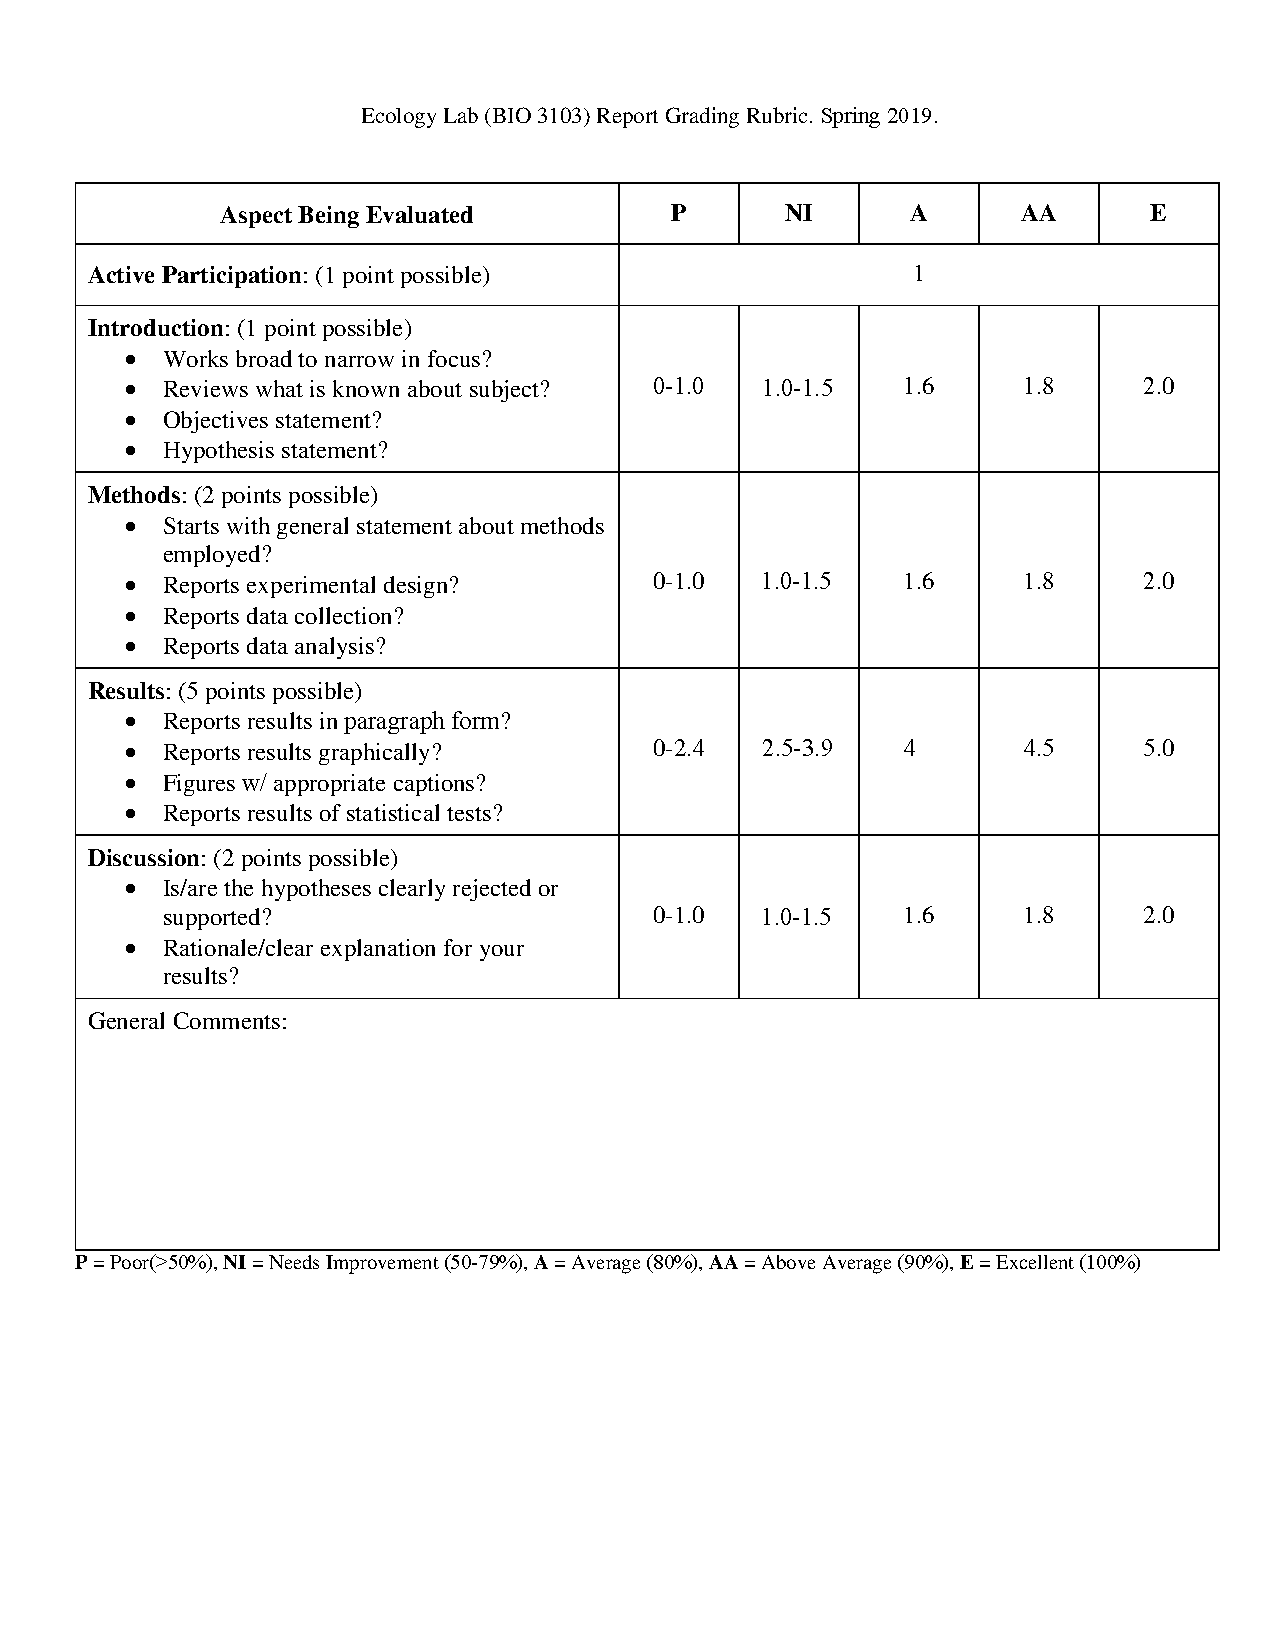
\includegraphics{Grading_rubric.pdf}
\caption{Grading rubric for Ecology Lab of Fall 2018. Each section will
be scored by the criteria provided under `Aspect being evaluated', and
points will total to 12 points.}
\end{figure}




\end{document}

\makeatletter
\def\@maketitle{%
  \newpage
%  \null
%  \vskip 2em%
%  \begin{center}%
  \let \footnote \thanks
    {\fontsize{18}{20}\selectfont\raggedright  \setlength{\parindent}{0pt} \@title \par}%
}
%\fi
\makeatother
